% vim: spelllang=fr

\documentclass[../main.tex]{subfiles}
\graphicspath{{\subfix{../Figures/Chap1/}}}
\begin{document}

\begin{itshape}
Ce premier chapitre introduit les cyclones tropicaux (TC), de la simple définition jusqu'à la formulation de la question scientifique présentée dans cette thèse, en introduisant tous les concepts intermédiaires nécessaires.
\end{itshape}

\minitoc
%----------------------------------------------------------------------------
\section{Introduction aux cyclones tropicaux}

\subsection{Qu'est-ce qu'un cyclone tropical}

Du grec \textit{κύκλος}, nom commun désignant un cercle, ou plus généralement toute chose circulaire ou ronde, le terme cyclone, dans un contexte météorologique, fait référence au type de circulation atmosphérique dans lequel l'air se trouve en rotation atour d'un centre de basse pression. Sous cette définition, le terme de cyclone désigne une grande quantité d'objets aux caractéristiques très diverses et prenant place à différentes échelles spatiales. Ainsi, à la
méso-échelle, caractérisée par des distances de l'ordre kilométrique, on peut notamment citer les méso-cyclones, vortex d'air ascendant et convergeant, mesurant généralement moins de \SI{10}{\kilo\metre} de diamètre et étant constituant notamment des orages super-cellulaires. De l'autre côté du spectre, à l'échelle synoptique, c'est à dire à l'échelle traitant des distances de l'ordre du millier de kilomètres, les plus grands objets météorologiques dépressionnaires pouvant être qualifiés de cyclones sont sans
nulle doute les vortex polaires ; de larges régions englobant chacune un pôle planétaire et dans laquelle de l'air froid est en rotation. Malgré ces différences apparentes, tous les cyclones possèdent néanmoins des caractéristiques communes. Ainsi, le centre du cyclone est toujours l'endroit où la pression atmosphérique est la plus faible, et la circulation de l'air autour du centre est assurée à minima par l'équilibre entre la force induite par le gradient de pression radial d'une part, et la somme
de la force centrifuge ainsi que la force de Coriolis d'autre part -- équilibre qualifié de cyclostrophique. La force de Coriolis, force inertielle causée par la rotation de la Terre, est également la raison pour laquelle les cyclones tournent dans le sens contraire des aiguilles d'une montre dans l'hémisphère nord, et inversement dans l'hémisphère sud.

Les cyclones tropicaux -- que l'on abrègera ensuite par l'acronyme TC, selon l'appellation anglaise \textit{Tropical Cyclone} -- sont un type de cyclone appartenant à l'échelle synoptique et qui ont la particularité de posséder un cœur chaud en haute troposphère. Le qualificatif de \textquote{tropical} fait référence à leur région d'origine, située dans la ceinture tropicale, définie en toute rigueur comme la zone située entre le Tropique du Cancer dans l'hémisphère nord et le Tropique du Capricorne dans
l'hémisphère sud (\ang{23;26;17.231} Nord et Sud, respectivement), et parfois approximée par la bande \ang{+20}~\ang{-20}~N. 

\begin{figure}[htpb]
    \centering
    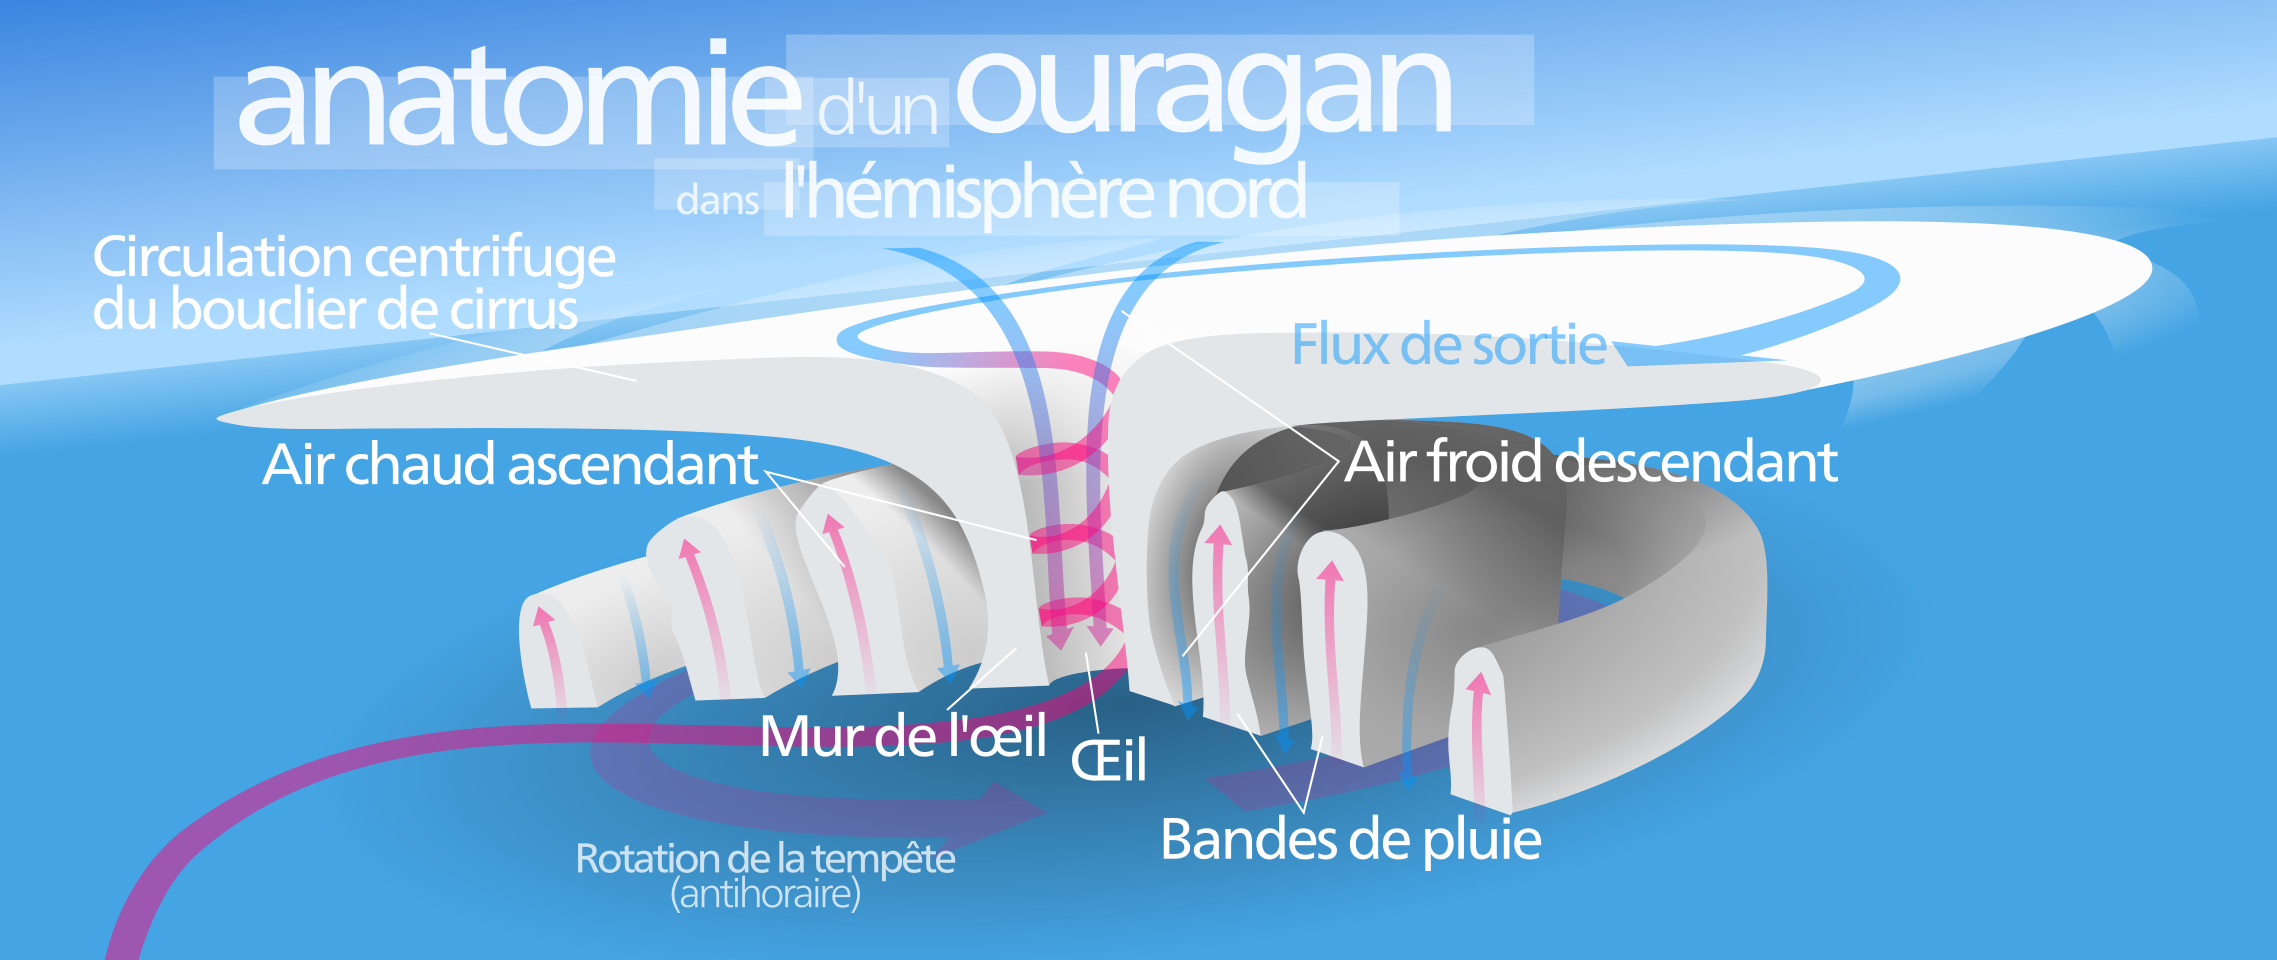
\includegraphics[width=\textwidth]{Hurricane-fr.png}
    \caption{By Kelvinsong - Own work, CC BY-SA 3.0, \url{https://commons.wikimedia.org/w/index.php?curid=23563610}}
    \label{fig:}
\end{figure}

Test de citation \cite{chauvin_response_2006}

\subsection{Bassins d'activité et saisonnalité}

\subsection{Risques associés et enjeux}

%-------------------------------------------------------------------------------
\section{Ingrédients de la cyclogénèse}
  
\subsection{Conditions de formation}

\subsection{Modèles conceptuels de fonctionnement}

\subsubsection{CISK}

\subsubsection{WISHE}

%-------------------------------------------------------------------------------
\section{Cyclones tropicaux et changement climatique}

\subsection{Bases de données observationelles}

\subsection{Les cyclones dans les modèles de climat}

\subsection{Consensus actuel sur les projections futures}

\subsection{Détection objective v.s indices de cyclogénèse}

%-------------------------------------------------------------------------------
\section{Synthèse}

\end{document}
